\documentclass[]{elsarticle} %review=doublespace preprint=single 5p=2 column
%%% Begin My package additions %%%%%%%%%%%%%%%%%%%

\usepackage[hyphens]{url}


\usepackage{graphicx}
%%%%%%%%%%%%%%%% end my additions to header

\usepackage[T1]{fontenc}
\usepackage{lmodern}
\usepackage{amssymb,amsmath}
% TODO: Currently lineno needs to be loaded after amsmath because of conflict
% https://github.com/latex-lineno/lineno/issues/5
\usepackage{lineno} % add
\usepackage{ifxetex,ifluatex}
\usepackage{fixltx2e} % provides \textsubscript
% use upquote if available, for straight quotes in verbatim environments
\IfFileExists{upquote.sty}{\usepackage{upquote}}{}
\ifnum 0\ifxetex 1\fi\ifluatex 1\fi=0 % if pdftex
  \usepackage[utf8]{inputenc}
\else % if luatex or xelatex
  \usepackage{fontspec}
  \ifxetex
    \usepackage{xltxtra,xunicode}
  \fi
  \defaultfontfeatures{Mapping=tex-text,Scale=MatchLowercase}
  \newcommand{\euro}{€}
\fi
% use microtype if available
\IfFileExists{microtype.sty}{\usepackage{microtype}}{}
\usepackage[margin=3cm]{geometry}
\usepackage[]{natbib}
\bibliographystyle{plainnat}

\ifxetex
  \usepackage[setpagesize=false, % page size defined by xetex
              unicode=false, % unicode breaks when used with xetex
              xetex]{hyperref}
\else
  \usepackage[unicode=true]{hyperref}
\fi
\hypersetup{breaklinks=true,
            bookmarks=true,
            pdfauthor={},
            pdftitle={},
            colorlinks=false,
            urlcolor=blue,
            linkcolor=magenta,
            pdfborder={0 0 0}}

\setcounter{secnumdepth}{0}
% Pandoc toggle for numbering sections (defaults to be off)
\setcounter{secnumdepth}{0}


% tightlist command for lists without linebreak
\providecommand{\tightlist}{%
  \setlength{\itemsep}{0pt}\setlength{\parskip}{0pt}}




\usepackage{booktabs}
\usepackage{longtable}
\usepackage{array}
\usepackage{multirow}
\usepackage{wrapfig}
\usepackage{float}
\floatplacement{figure}{H}
\newcommand{\pandocbounded}[1]{#1}
\usepackage{colortbl}
\usepackage{pdflscape}
\usepackage{tabu}
\usepackage{threeparttable}
\usepackage{threeparttablex}
\usepackage[normalem]{ulem}
\usepackage{makecell}
\usepackage{xcolor}
\usepackage{booktabs}
\newcommand{\blandscape}{\begin{landscape}}
\newcommand{\elandscape}{\end{landscape}}
\usepackage{float} \floatplacement{figure}{H}
\newcommand{\beginsupplement}{\setcounter{table}{0}  \renewcommand{\thetable}{S\arabic{table}}     -   - \setcounter{figure}{0} \renewcommand{\thefigure}{S\arabic{figure}}}
\usepackage{booktabs}
\usepackage{longtable}
\usepackage{array}
\usepackage{multirow}
\usepackage{wrapfig}
\usepackage{float}
\usepackage{colortbl}
\usepackage{pdflscape}
\usepackage{tabu}
\usepackage{threeparttable}
\usepackage{threeparttablex}
\usepackage[normalem]{ulem}
\usepackage{makecell}
\usepackage{xcolor}



\begin{document}


\begin{frontmatter}

  \title{}
    \author[1]{Andrew Lowther%
  %
  }
  
    \author[2]{Ulf Lindstrøm%
  %
  }
  
    \author[3]{Bjørn Krafft%
  %
  }
  
    \author[4]{Javier A. Arata%
  %
  }
  
      \cortext[cor1]{Corresponding author}
  
  \begin{abstract}
  
  \end{abstract}
  
 \end{frontmatter}

\subsection{Tables}\label{tables}

Table 1: Estimates of mean imputed summer LKB for +/- SAM summer index,
a per equation (2).

\subsection{Figures}\label{figures}

\begin{verbatim}
• Figure 1: Impact of Spatial and Temporal Adjustments on Expected Penguin Performance. Illustrate the combined effect of spatial and temporal corrections on model outputs. Highlight that LHR impacts are overestimated in the original model.
\end{verbatim}

Content: • Boxplots~comparing expected penguin performance under: ◦
Original model~(gSSMU scales, Adélie/chinstrap penguins included in
winter, March as summer). ◦ Revised model~(SSMU scales, Adélie/chinstrap
penguins excluded in winter, March as winter). • Color-coded by ONI
conditions: ◦ Warm (≥0.5°C; red). ◦ Neutral (-0.5°C \textless{} ONI
\textless{} 0.5°C; white). ◦ Cold (\textless-0.5°C; blue).

\begin{verbatim}
• Table 1: Marginal Probabilities of Negative Impacts on Penguin Performance
\end{verbatim}

Content: • Comparison of marginal probabilities~for: ◦ Original
model~(Watters et al., 2020). ◦ Revised model~(spatial rescaling to
SSMU, temporal adjustments, March as winter). • What to include: •
Probability of negative impact from~high LHR~(original: 93\%; revised:
37\%). • Probability under~``Worst Case''~(neutral ONI, high LHR, high
LKB). • Dominance of~ONI effects~in revised model.

Unvalidated Ecological Assumptions • Figure 1: Relationship Between SAM
Phases and Local Krill Biomass (LKB). Visually confirm the~lack of
correlation~between SAM and LKB. Support the argument that~local
processes~(e.g., upwelling, bathymetry) are more influential than
broad-scale climate indices. Content: • Scatter plots or regression
plots~showing: ◦ SAM index values~(x-axis) vs.~Local Krill Biomass
(LKB)~(y-axis). ◦ Data points~for different SAM phases (positive,
neutral, negative). ◦ Regression line~with~R² and p-values~indicating no
significant relationship (F \textless{} 0.975, p \textgreater{} 0.33). •
Highlight:~Visual demonstration that~LKB does not vary predictably with
SAM phases.

\begin{verbatim}
• Table 1: Statistical Tests for SAM-LKB and Low LKB-Small Krill Relationships
\end{verbatim}

Content:

\begin{table}[ht]
\centering
\resizebox{\textwidth}{!}{%

\begin{tabular}{lccc}
\toprule
Statement/Question & Data Source & Support \& Significance & Conclusions\\
\midrule
Does LKB vary with SAM sign and strata ? & Appendix I & No; F < 0.975, p >0.33 all cases & LKB does not vary predictably with SAM\\
Is low LKB (<1Mt) correlated with small krill ? & Appendix II & No; F < 2.175, p >0.154 all cases & Low LKB in Best Case scenario is inappropriate\\
Are penguin indices related to ONI/SAM ? & Appendix III & No; see Appendix III Table 1 & Penguin indices are not correlated to climate variability indices\\
\bottomrule
\end{tabular}
}
\caption{Summary Table showing what was bullshit, and where to find the analysis and data in our paper.}
\end{table}

\begin{figure}
\includegraphics[width=0.65\linewidth]{./Watters EMM figures/Penguin distributions} \caption{Penguin foraging behaviour during summer breeding, derived from available ARGOS-CLS PTT data presented in Hinke et al. 2017. A) Chinstrap penguins from Cape Shireff (blue) and Copacabana (green) truncated at $10^{th}$ March in line with known phenology (Black 2016).  Elongated grey track represents a single animal) B) Adélie penguins truncated to the end of January and C) gentoo penguins until \textasciitilde{}August, representing all available PTT data provided. The SSMU are combined and coloured according to gSSMU (red; gSSMU 2, purple; gSSMU 1) with chinstrap and Adélie penguin 99\% MCP home ranges occupying between 7-19\% of the gSSMU to which they were assigned.}\label{fig:Penguin distribution plots}
\end{figure}

\begin{figure}
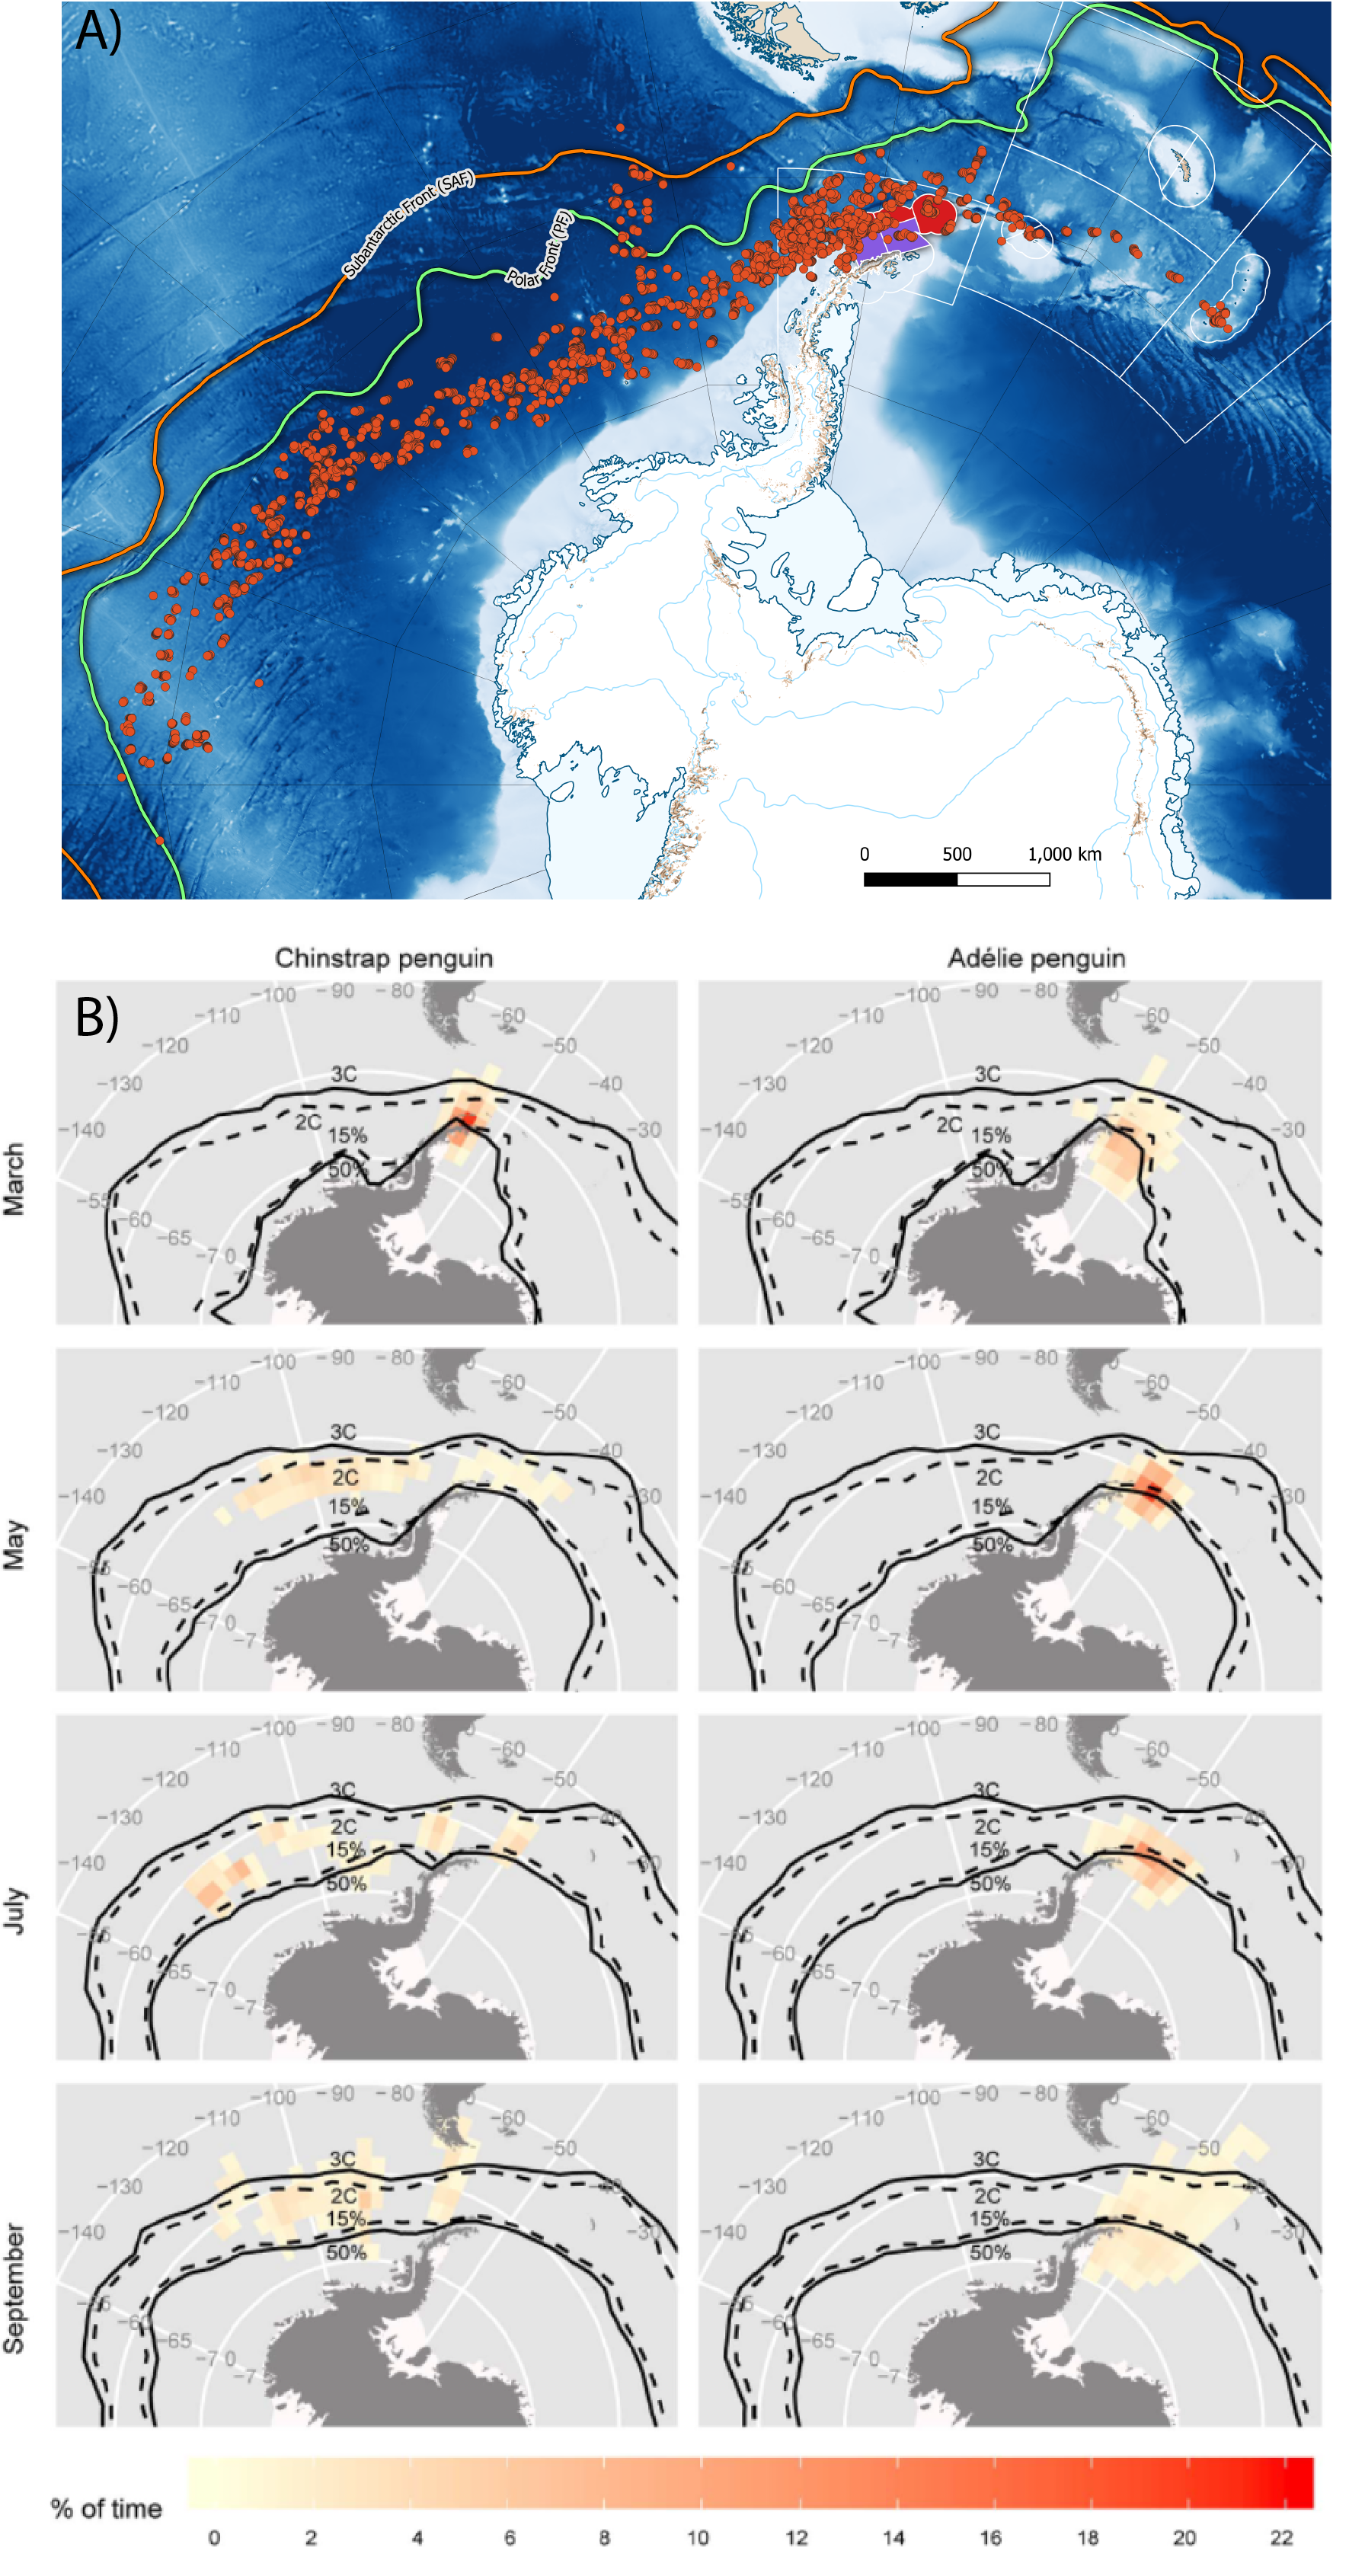
\includegraphics[width=0.75\linewidth]{./Watters EMM figures/Overwinter pengo distributions} \caption{A) Distribution of overwinter movement for chinstrap penguins, relative to the gSSMU's to which they were attributed, created from telemetry data available in Hinke et al. 2019.  B) Adélie and chinstrap penguin movement recorded by light geolocators, highlighting the large longitudinal range both species disperse through at the end of breeding (taken from Hinke et al. 2015).  In the original model formulation by Watters et al. 2020, the winter performance indices for both species are matched to macroscale levels of ONI variability but gSSMU-scale estimates of LKB and LHR.}\label{fig:Overwinter penguin  plots}
\end{figure}

\begin{figure}
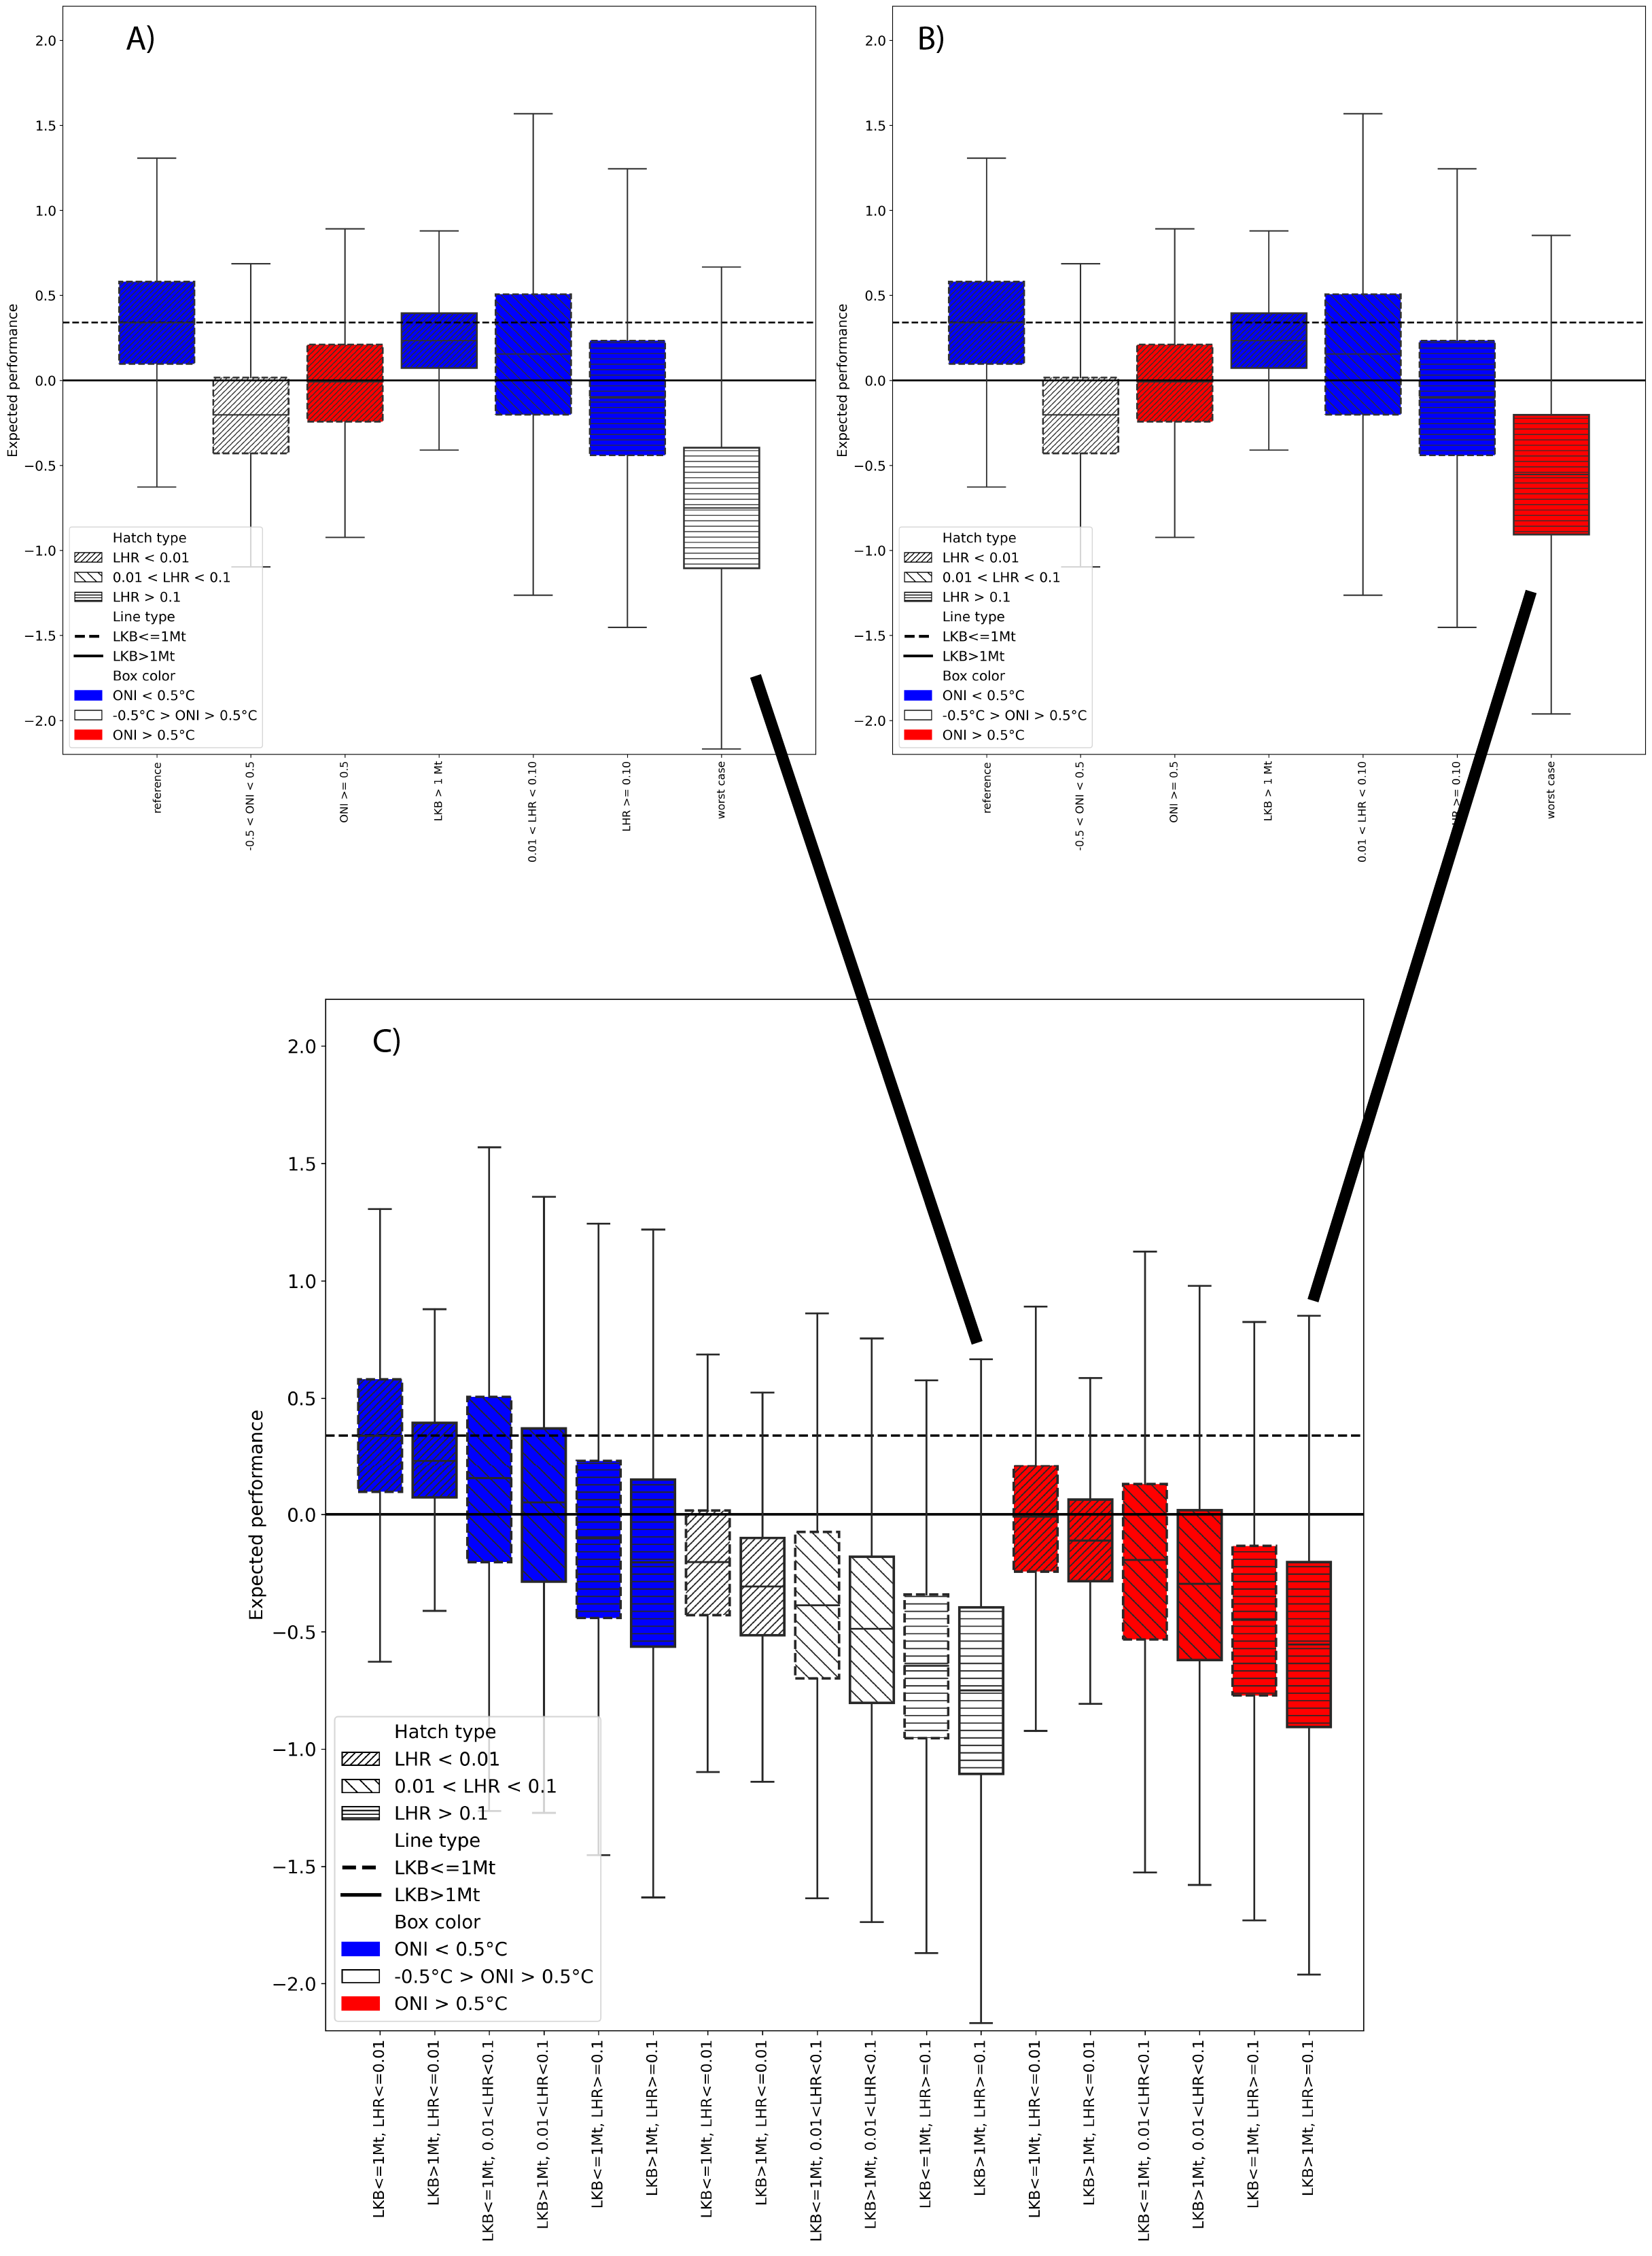
\includegraphics[width=0.75\linewidth]{./Watters EMM figures/Watters original and mistake} \caption{Original Figure 1 plot from Watters et al. 2020 with A) Neutral ONI and B) B) Warm ONI constituting the Worst Case selected.  C) Displays the original case-by-case plots recreated from the paper, with Case 12 representing the intention while data from Case 18 was selected for rendering the boxplot.  Note that the expected performance under neutral ONI Worst Case is poorer than under the warm ONI that was presented in the original paper.  Henceforth, to facilitate comparison, we refer to the ONI Neutral plot however we consider this unrealistic if the intention is to portray a Worst Case of a continuing warming climate.}\label{fig:Watters original and mistake}
\end{figure}

\begin{figure}

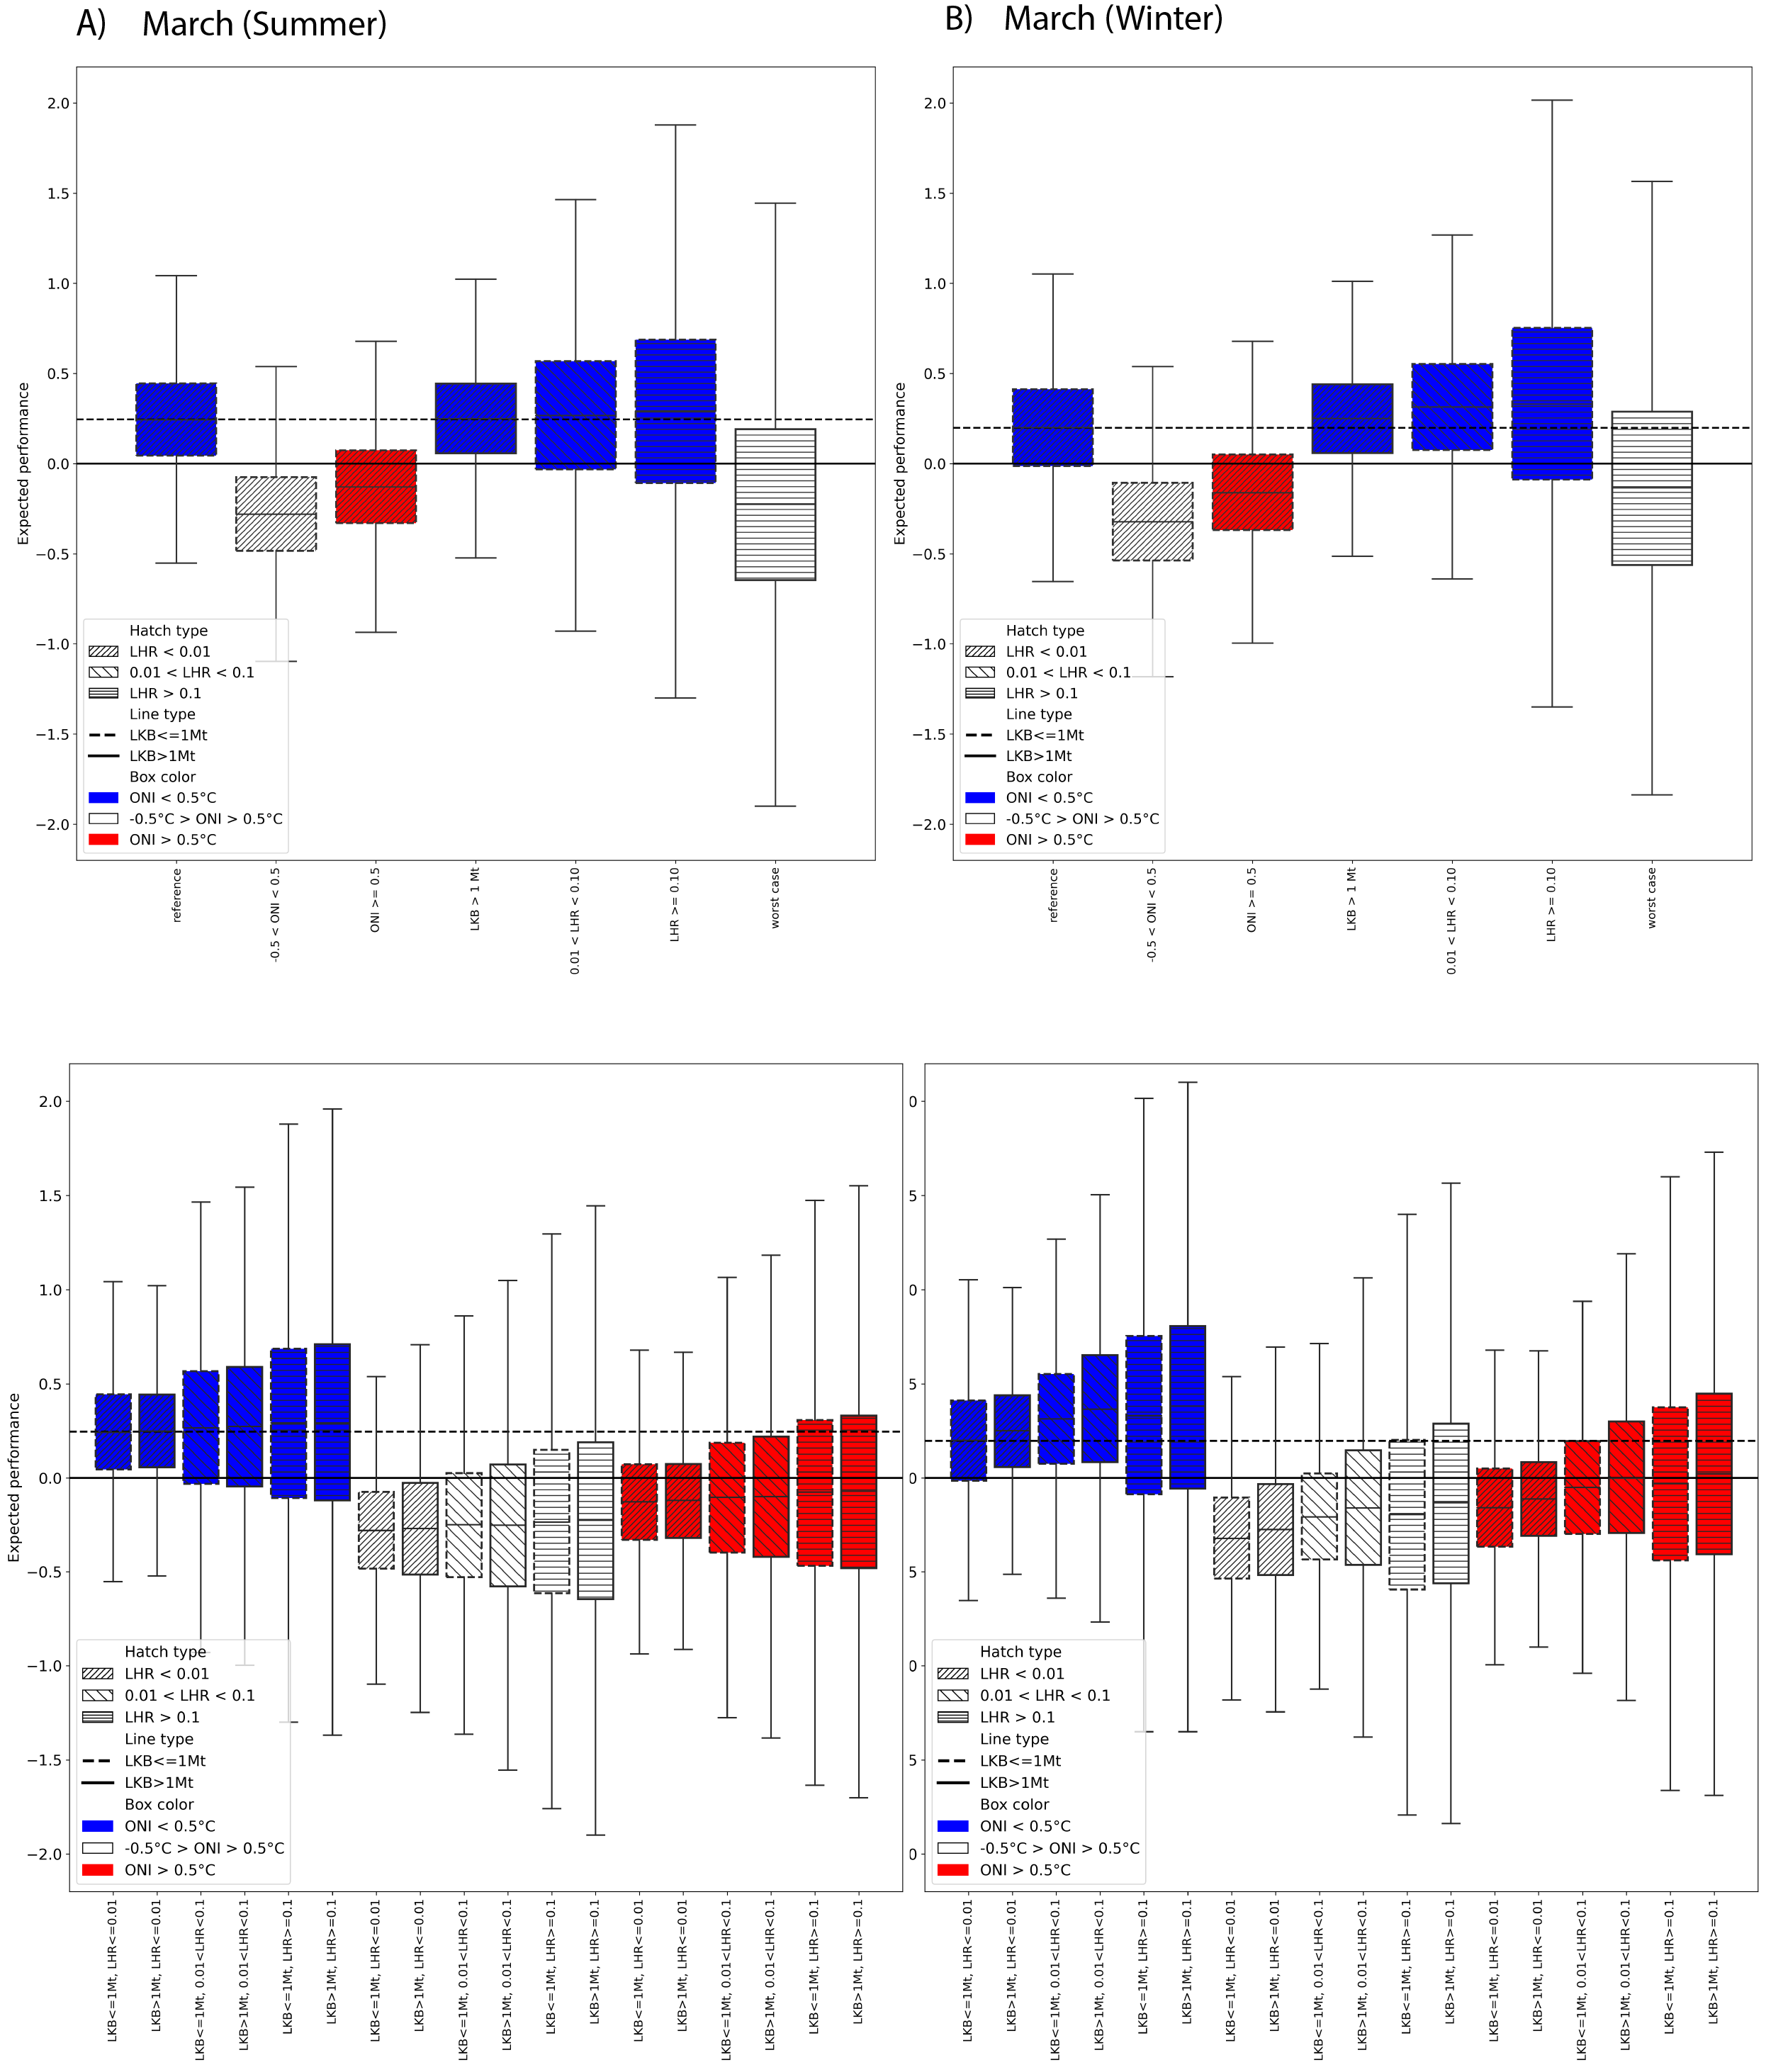
\includegraphics[width=1\linewidth]{./Watters EMM figures/All spp summer then winter 37} \hfill{}

\caption{Model output for the alternatve Watters et al. 2020 scenario outlined above (all species initially present, Adélie and chinstrap penguins migrate out of the area after breeding, LKB and LHR rescaled to SSMU and March included in summer or winter).   Selected cases as per Watters et al. 2020 for March in A) Summer and B) Winter are provided, with the corresponding case-by-case boxplots presented beneath.  Boxplots are colour-coded by ONI state (red=warm, white=neutral, blue=cold).  In all cases, the marginal effect of ONI dominated the expected performance of penguins against their long-term mean, irrespective of LKB or LHR.}\label{fig:Scenario plot 1}
\end{figure}

\begin{landscape}

\begin{longtable}[t]{lccccc}
\caption{\label{tab:Table 1 Scenario Original}Original table in Watters et al. 2020.  In this and all subsequent tables below, the posterior and posterior predictive probabilities that the expected performance of penguins given the effects in the left hand column are less than the expected performance given the drivers in the column headings are provided. Worst Case is represented by neutral ONI; LHR  $\geqslant$ 0.1; and LKB $\geqslant$ 1Mt.  The Best Case is represented by La Niña conditions, low LKB and low LHR.}\\
\toprule
Effects & Best Case & -0.5°C < ONI < +0.5°C & ONI > +0.5°C & Long-term µ & Long-term predicted µ\\
\midrule
Best case & NA & NA & NA & 0.04 & 0.36\\
ONI Neutral & 1.00 & NA & NA & 0.89 & 0.59\\
ONI warm & 0.99 & NA & NA & 0.52 & 0.51\\
LKB High & 0.71 & 0.02 & 0.12 & 0.01 & 0.41\\
LHR medium & 0.75 & 0.16 & 0.31 & 0.32 & 0.44\\
\addlinespace
LHR high & 0.93 & 0.39 & 0.61 & 0.64 & 0.54\\
Worst case & 0.99 & NA & NA & 0.99 & 0.78\\
\bottomrule
\end{longtable}

\begin{longtable}[t]{lccccc}
\caption{\label{tab:Table 1 Scenario 37a}Posterior and posterior predictive probabilities extracted from the model output for alternatve Watters et al. 2020 scenario outlined above with March attributed to winter (Adélie and chinstrap penguins migrate out of the area after breeding, LKB and LHR rescaled to SSMU). Under this scenario, performance against the long term mean is worst for neutral and warm ONI conditions.}\\
\toprule
Effects & Best Case & -0.5°C < ONI < +0.5°C & ONI > +0.5°C & Long-term µ & Long-term predicted µ\\
\midrule
Best case & NA & NA & NA & 0.04 & 0.40\\
ONI Neutral & 1.00 & NA & NA & 0.97 & 0.62\\
ONI warm & 0.99 & NA & NA & 0.81 & 0.56\\
LKB High & 0.49 & 0.01 & 0.05 & 0.03 & 0.40\\
LHR medium & 0.46 & 0.04 & 0.09 & 0.14 & 0.39\\
\addlinespace
LHR high & 0.45 & 0.10 & 0.16 & 0.23 & 0.39\\
Worst case & 0.84 & NA & NA & 0.71 & 0.59\\
\bottomrule
\end{longtable}

\elandscape
\blandscape

\begin{longtable}[t]{lccccc}
\caption{\label{tab:Table 1 Scenario 37b}Posterior and posterior predictive probabilities extracted from the model output for alternatve Watters et al. 2020 scenario outlined above with March attributed to summer (Adélie and chinstrap penguins migrate out of the area after breeding, LKB and LHR rescaled to SSMU). Under this scenario performance against the long term mean is also worst for neutral and warm ONI conditions.}\\
\toprule
Effects & Best Case & -0.5°C < ONI < +0.5°C & ONI > +0.5°C & Long-term µ & Long-term predicted µ\\
\midrule
Best case & NA & NA & NA & 0.10 & 0.42\\
ONI Neutral & 1.00 & NA & NA & 0.98 & 0.63\\
ONI warm & 0.99 & NA & NA & 0.86 & 0.56\\
LKB High & 0.40 & 0.00 & 0.04 & 0.03 & 0.40\\
LHR medium & 0.27 & 0.01 & 0.02 & 0.04 & 0.37\\
\addlinespace
LHR high & 0.37 & 0.08 & 0.13 & 0.21 & 0.38\\
Worst case & 0.76 & NA & NA & 0.63 & 0.55\\
\bottomrule
\end{longtable}

\elandscape
\blandscape

\elandscape
\blandscape

\end{landscape}

\newpage
\beginsupplement
\blandscape

\section{Supplementary material}\label{supplementary-material}

\begin{figure}
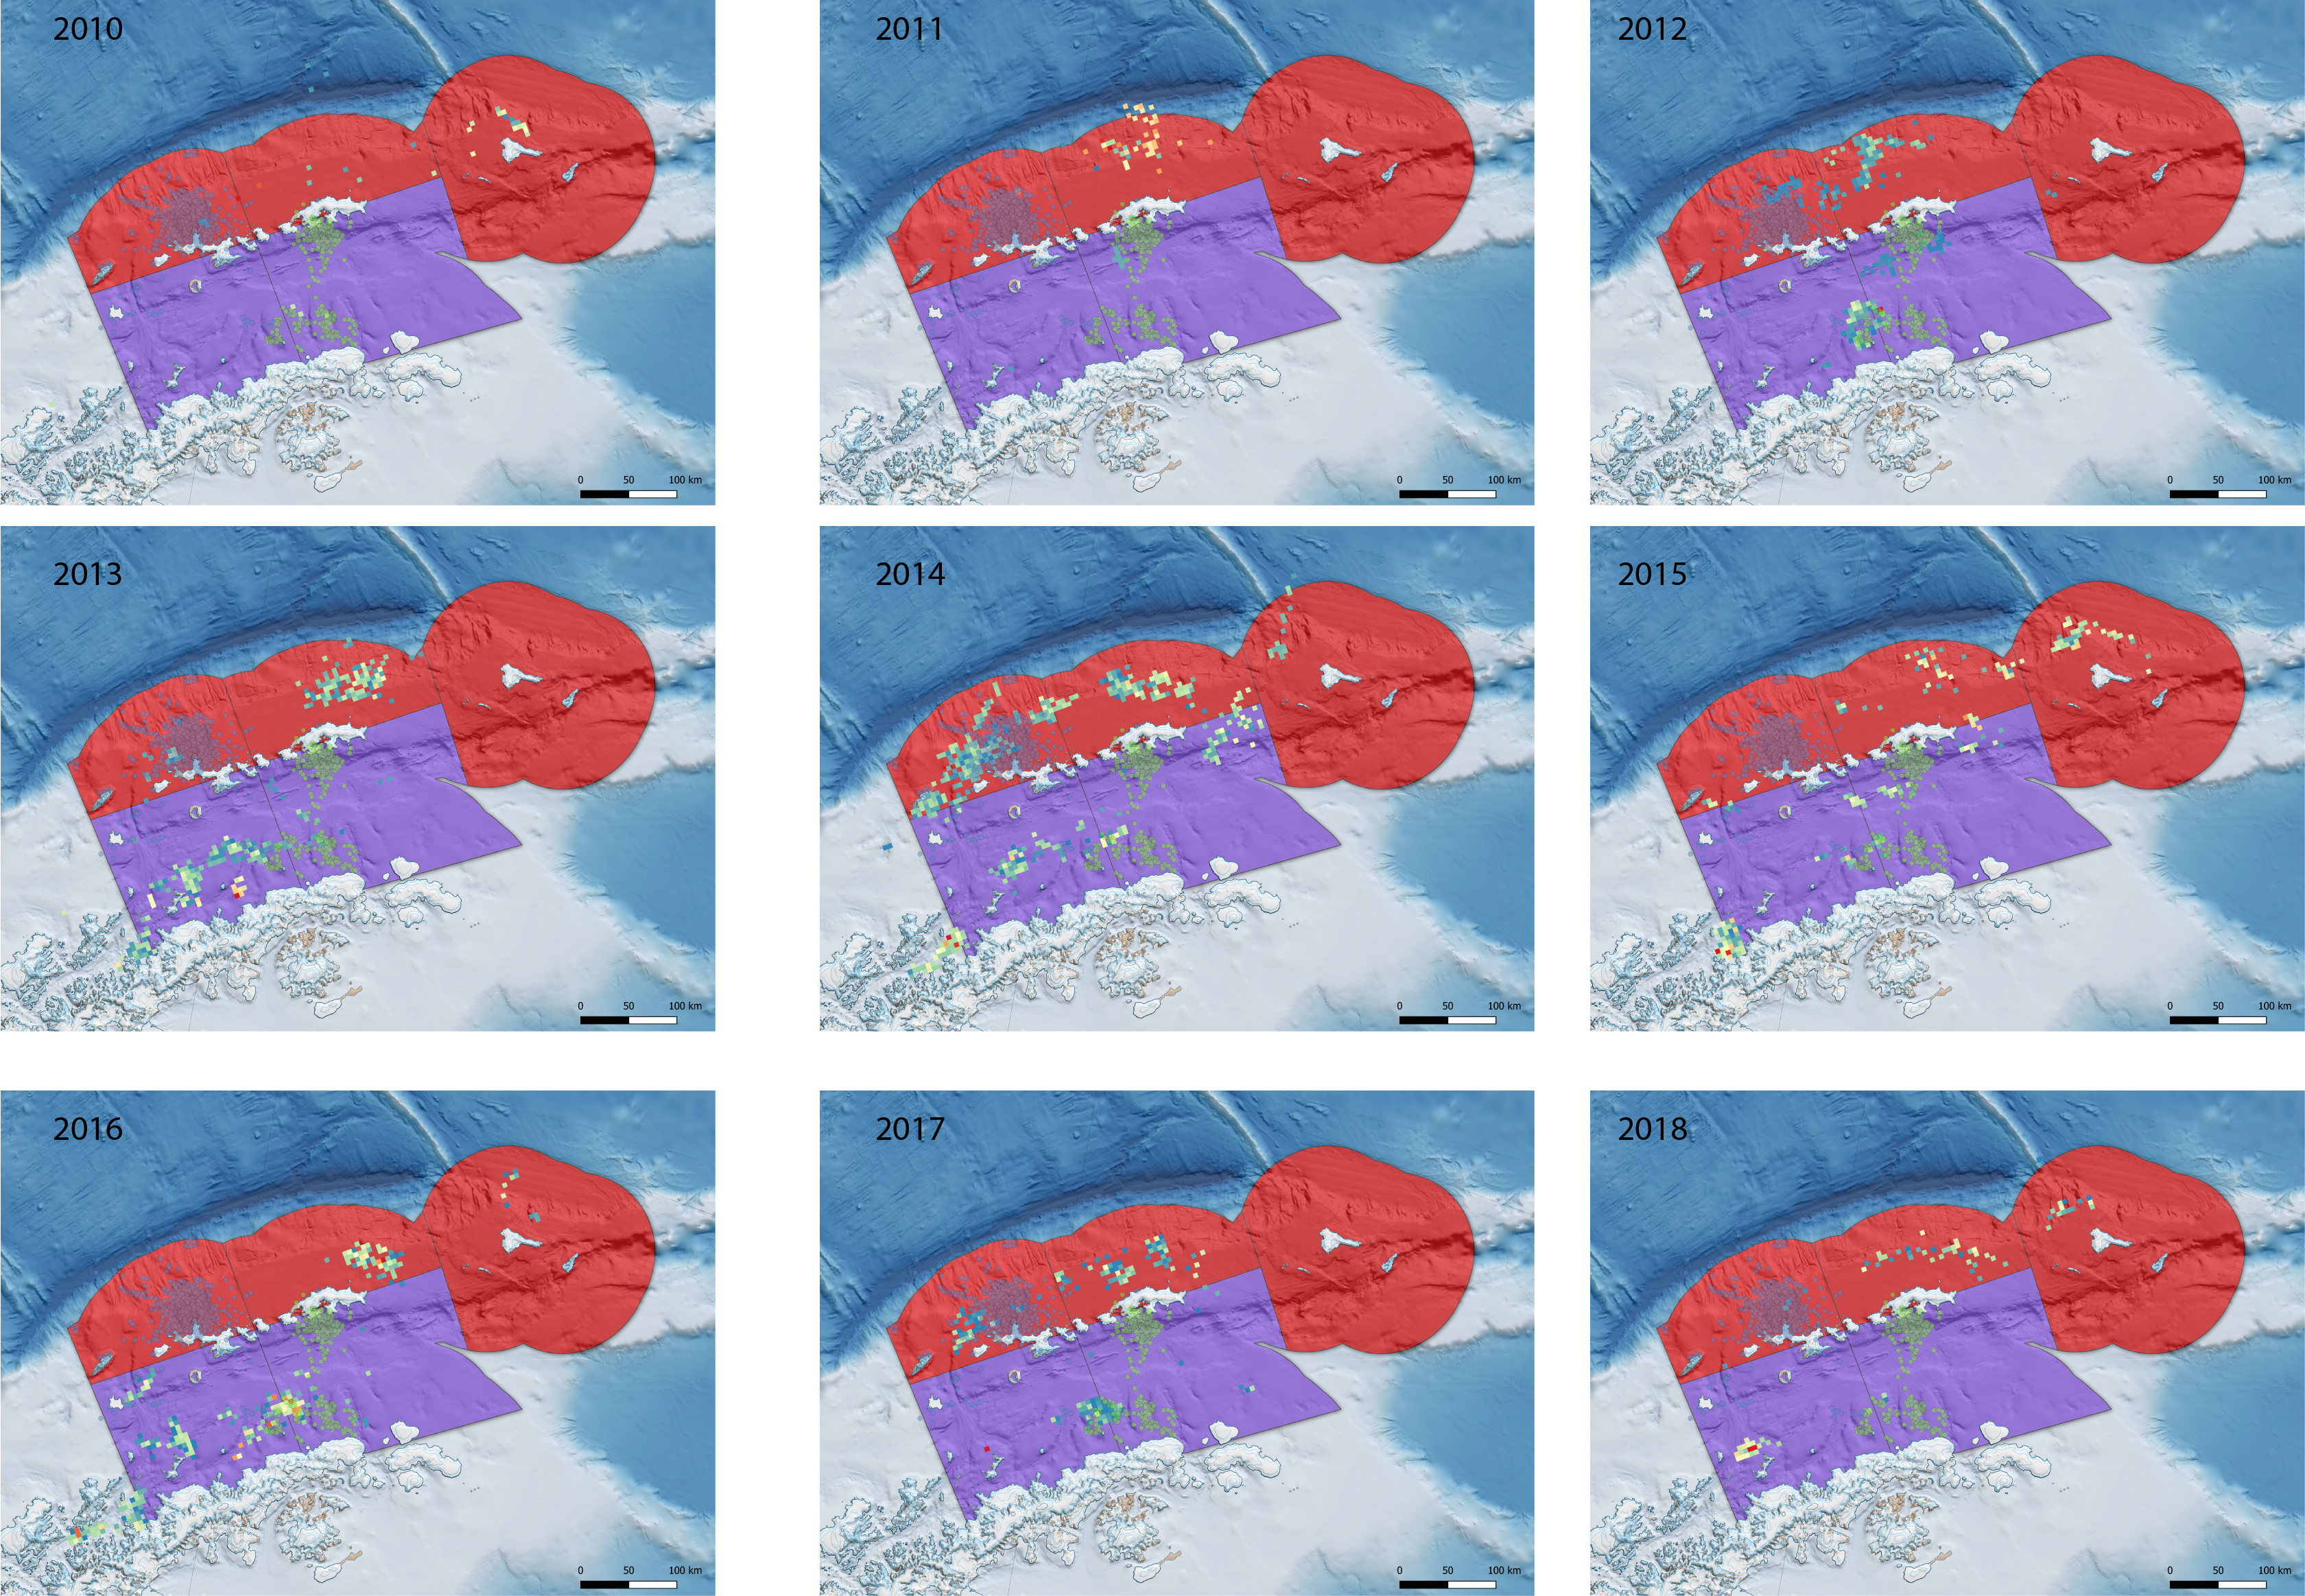
\includegraphics[width=0.8\linewidth]{./Watters EMM figures/summer catch/Year by year catch} \caption{C1 Catch and Effort data for 2010 - 2018, for all catches during the period of the austral summer relating to Adélie and chinstrap penguins in Subarea 48.1 (i.e. up to $10^{th}$ March).  The telemetry data presented in Hinke et al. 2017 for chinstrap penguins at both Cape Shireff and Copacabana and the gSSMU used in the Watters et al. 2020 paper are superimposed to highlight the extreme variability in actual catch, relative to the scale of LHR used to reflect interactions with penguins.  Our reanalysis re-scaled LHR to the SSMU level, though we contend that for the purposes of matching predator data at appropriate spatial scales even this is too coarse a resolution.}\label{fig:Supplementary Figure 1}
\end{figure}

\end{landscape}

\begin{figure}

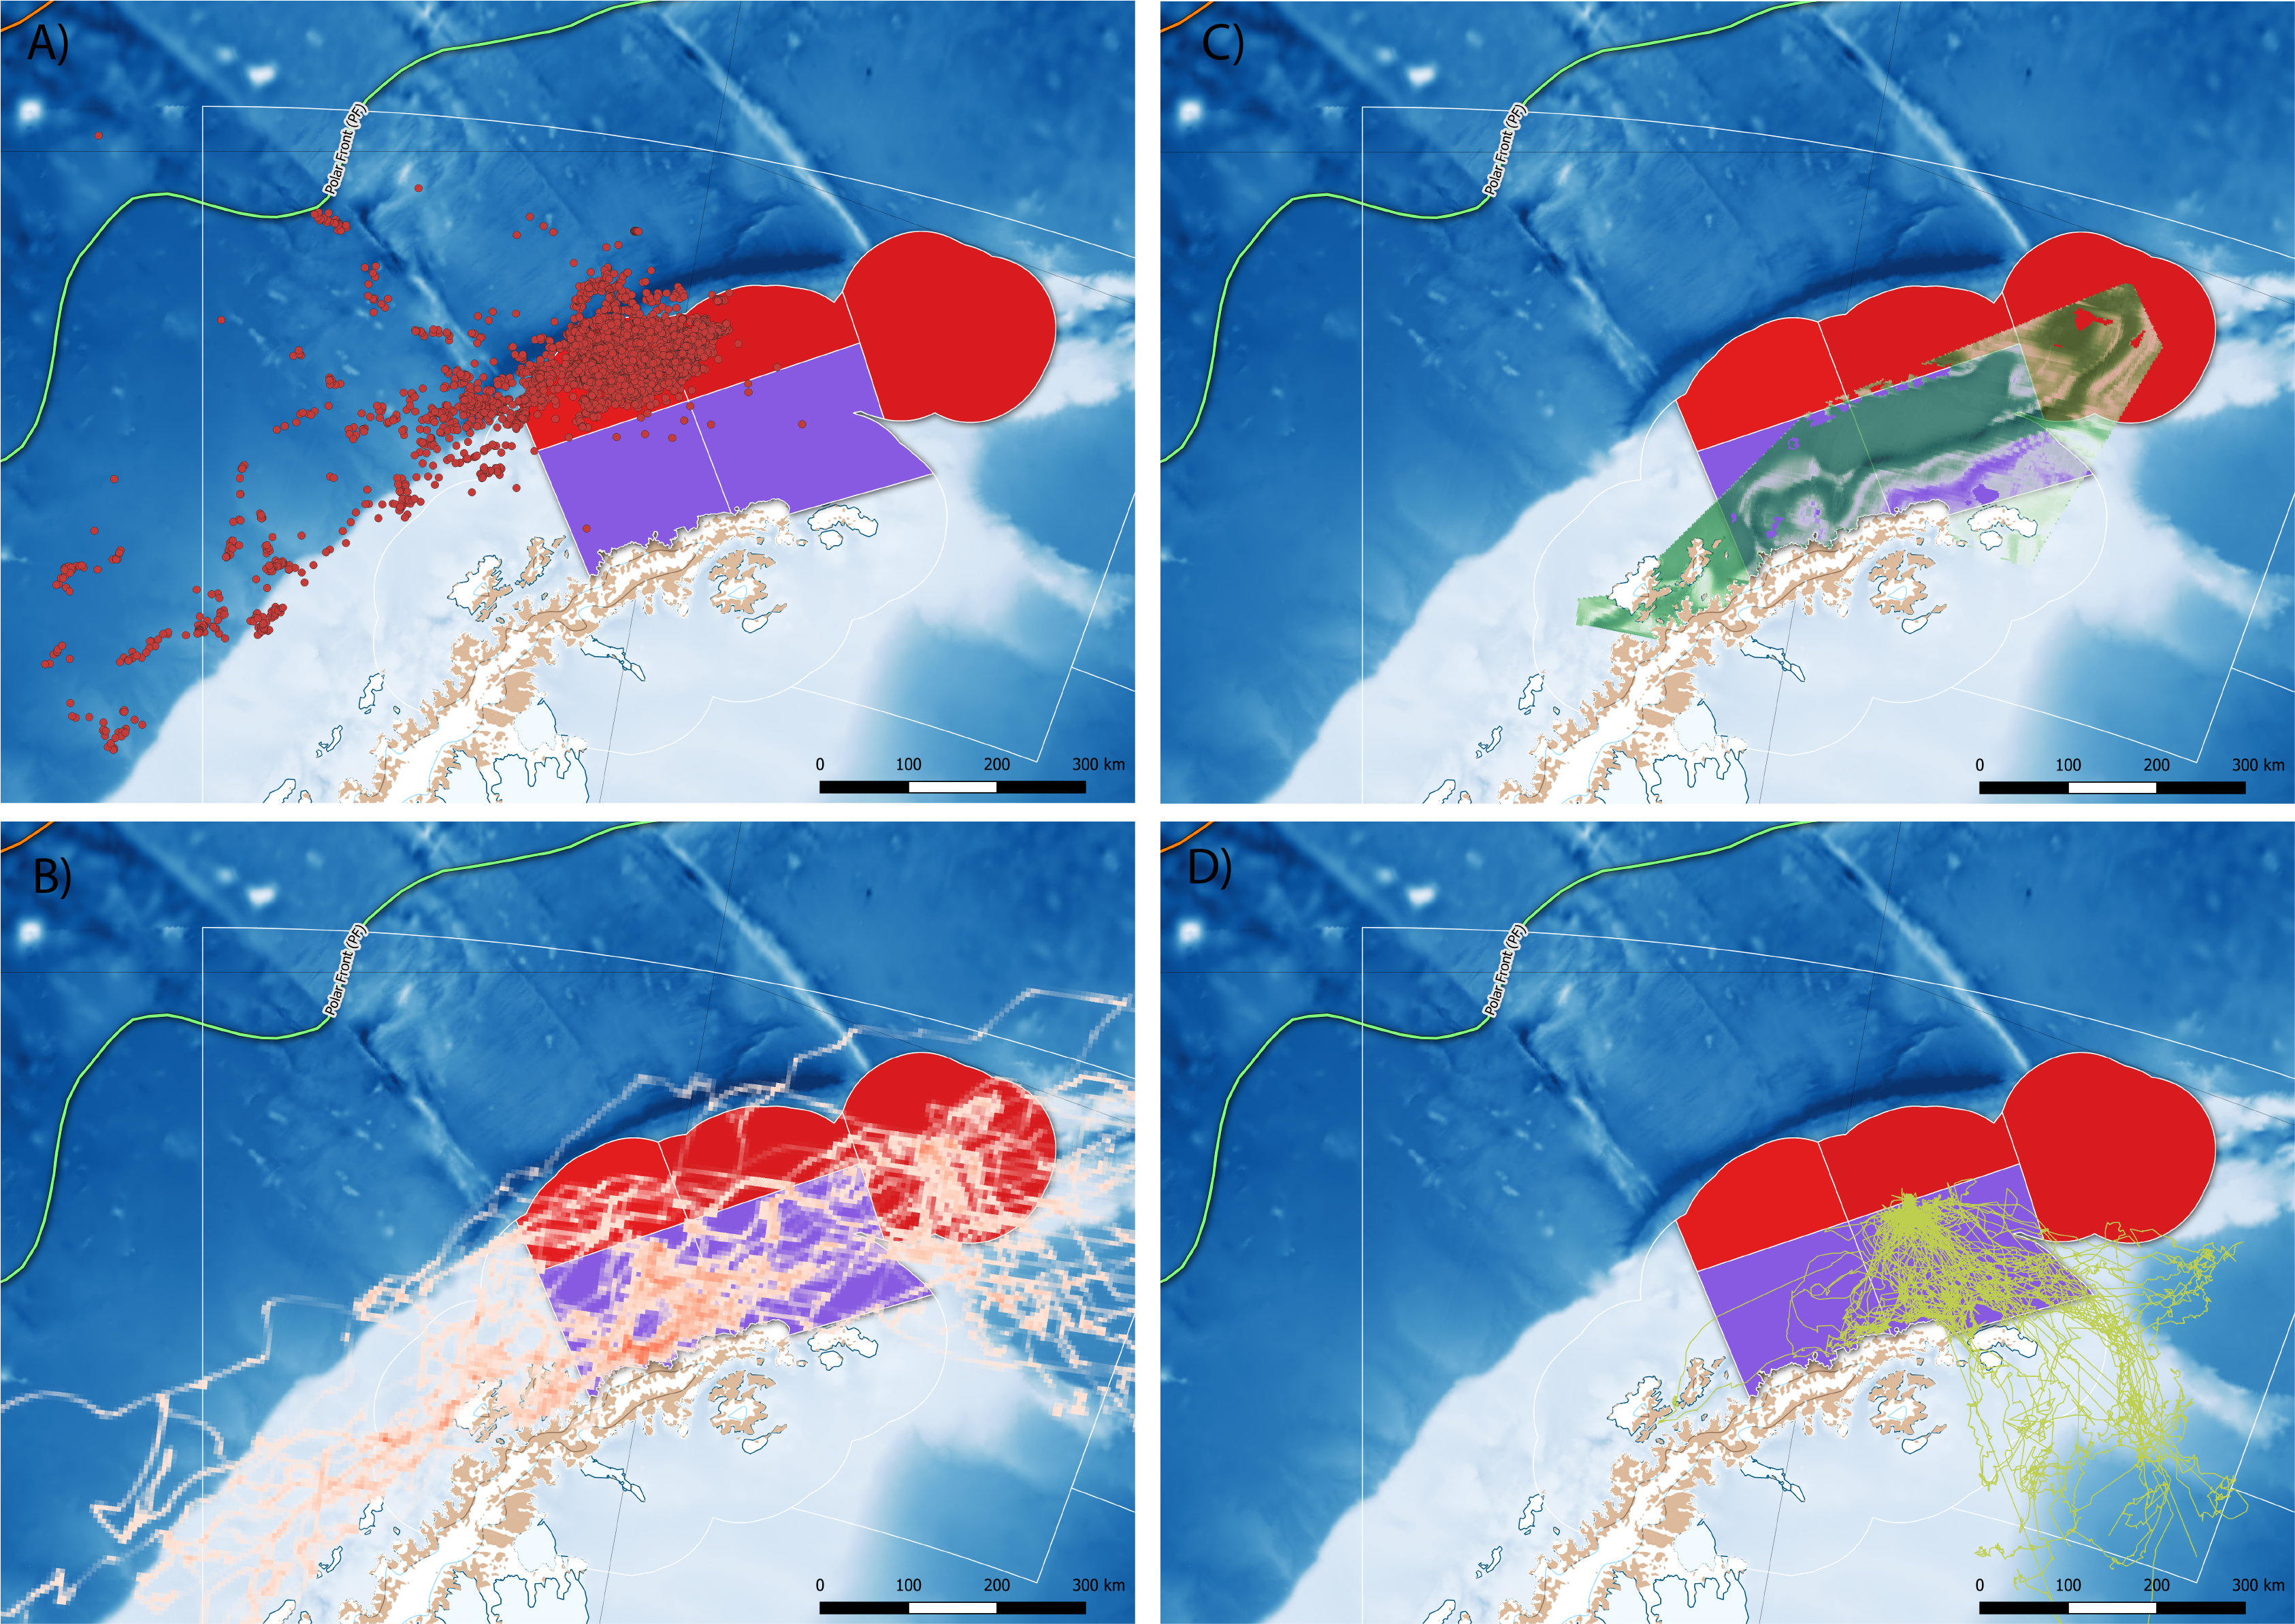
\includegraphics[width=1\linewidth]{./Watters EMM figures/Other spp distribution} \hfill{}

\caption{The summer distribution of foraging effort by A) adult female Antarctic fur seals (adapted from telemetry data available in Hinke et al. 2017), B) migratory adult male Antarctic fur seals (adapted from Lowther et al. 2020) C) humpback whales throughout December (adapted from Johannessen et al., this meeting) and D) nonbreeding adult Adélie penguins during the breeding season (adapted from data in Oosthuizen et al., this meeting). Potential effects of competitive overlap between pygoscelid penguins and other krill dependent predators, particularly those who have increased their abundance dramatically over the preceding 40 years, are excluded from both approaches, creating an unrealistic set of boundary conditions for interpreting the variance in penguin vital rates.}\label{fig:Supplementary Figure 2 other species plots}
\end{figure}

\newpage

\renewcommand\refname{Citations}
\bibliography{mylib.bib}


\end{document}
